%% The "\appendix" call has already been made in the declaration
%% of the "appendices" environment (see thesis.tex).
\chapter{Miscellanious}
\section{Intersection Tester Doxygen Sample} \label{app:Pointless}

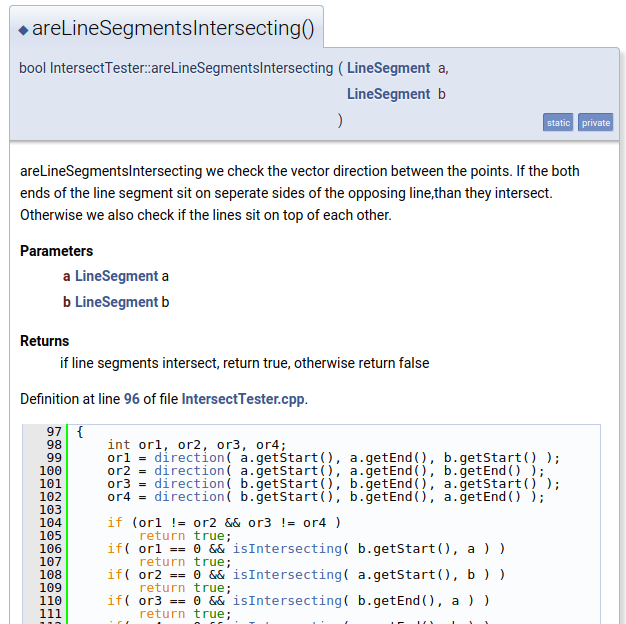
\includegraphics[width=1\textwidth]{images/softwareDevelopment}

\chapterquote{%
Le savant n'\'etudie pas la nature parce que cela est utile; \\
\indent il l'\'etudie parce qu'il y prend plaisir, \\
\indent et il y prend plaisir parce qu'elle est belle.}%
{Henri Poincar\'e, 1854--1912}

Appendixes (or should that be ``appendices''?) make you look really clever, 'cos
it's like you had more clever stuff to say than could be fitted into the main
bit of your thesis. Yeah. So everyone should have at least three of them\dots

\section{Like, duh}
\label{sec:Duh}
Padding? What do you mean?

\section{$y = \alpha x^2$}
\label{sec:EqnTitle}
See, maths in titles automatically goes bold where it should (and check the
table of contents: it \emph{isn't} bold there!) Check the source: nothing
needs to be specified to make this work. Thanks to Donald Arsenau for the
teeny hack that makes this work.

%% Big appendixes should be split off into separate files, just like chapters
%\input{app-myreallybigappendix}
